\documentclass[handout, red]{beamer}

%\documentclass[notes]{beamer}
%\documentclass[notes=hide]{beamer}
%\documentclass[notes=only]{beamer}

% Class options include: notes, notesonly, handout, trans,
%                        hidesubsections, shadesubsections,
%                        inrow, blue, red, grey, brown

% Theme for beamer presentation.
\usepackage{beamerthemelined} 
% Other themes include: beamerthemebars, beamerthemelined, 
%                       beamerthemetree, beamerthemetreebars  



\title{Making NHS IT less bad}    % Enter your title between curly braces
\author{Carl Reynolds\\}                 % Enter your name between curly braces
\institute{@drcjar/carlreynolds.net/openhealthcare.org.uk}      % Enter your institute name between curly braces
\date{}                    % Enter the date or \today between curly braces

\begin{document}

% Creates title page of slide show using above information
\begin{frame}
  \titlepage
\end{frame}
\note{Talk for 30 minutes} % Add notes to yourself that will be displayed when
                           % typeset with the notes or notesonly class options

%\section[Outline]{}

% Creates table of contents slide incorporating
% all \section and \subsection commands
\begin{frame}
  \tableofcontents
\end{frame}

\section{Intro, is there really a problem?}

\begin{frame}
 \begin{figure}[htp]
\centering
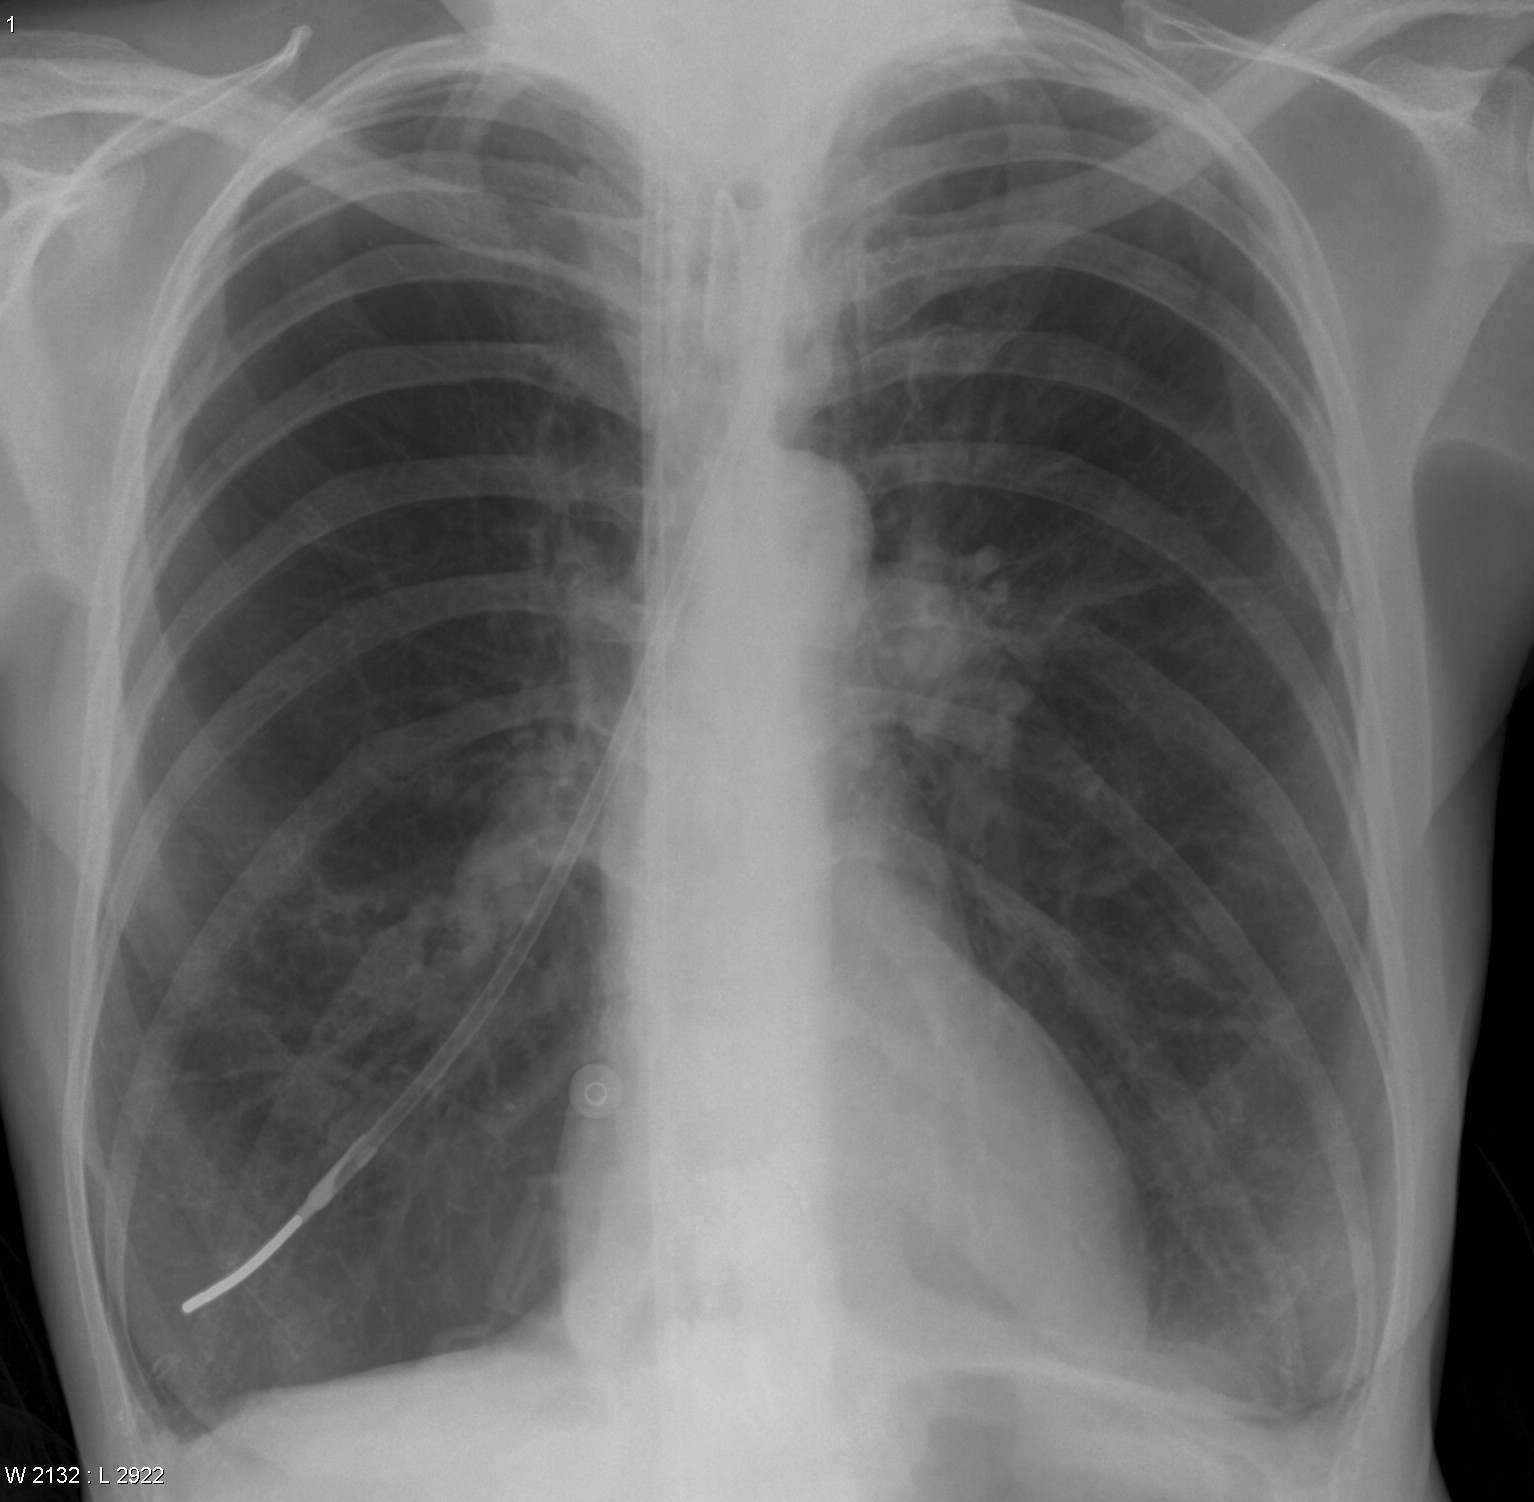
\includegraphics[width=8cm,height=7cm]{figs/ng_tube.jpg}
\caption{Is the naso-gastric tube in place? This a pass/fail question.}\label{fig:bugsa}
\end{figure}
 
 \end{frame}
 


\begin{frame}
  \frametitle{Three terrible tales of systems suboptimality..and a puzzle}   % Insert frame title between curly braces

  
  
 \begin{itemize}
 
 \item Three tales
 
 \begin{enumerate}
  \item Can't see the xrays (NG tubes and brain injury)
  
  \item Didn't see the camera test (system fragmentation)
  
  \item Communication breakdown it's always the same (lost to follow up, failed referral, broken fax machines)
  \end{enumerate}
  
 
   \item How did the receptionist fax the referral card that was too thick for the fax machine?
  \end{itemize}

\end{frame}

\begin{frame}
\begin{itemize}
  \item Surely people just file bug reports and this stuff gets fixed right?
  \item Closest we have to a bug reporting system is NRLS...
  \item What does NRLS show?
 \end{itemize}
\end{frame}	

\begin{frame}
  \frametitle{}   % Insert frame title between curly braces
  
\begin{figure}[htp]
\centering
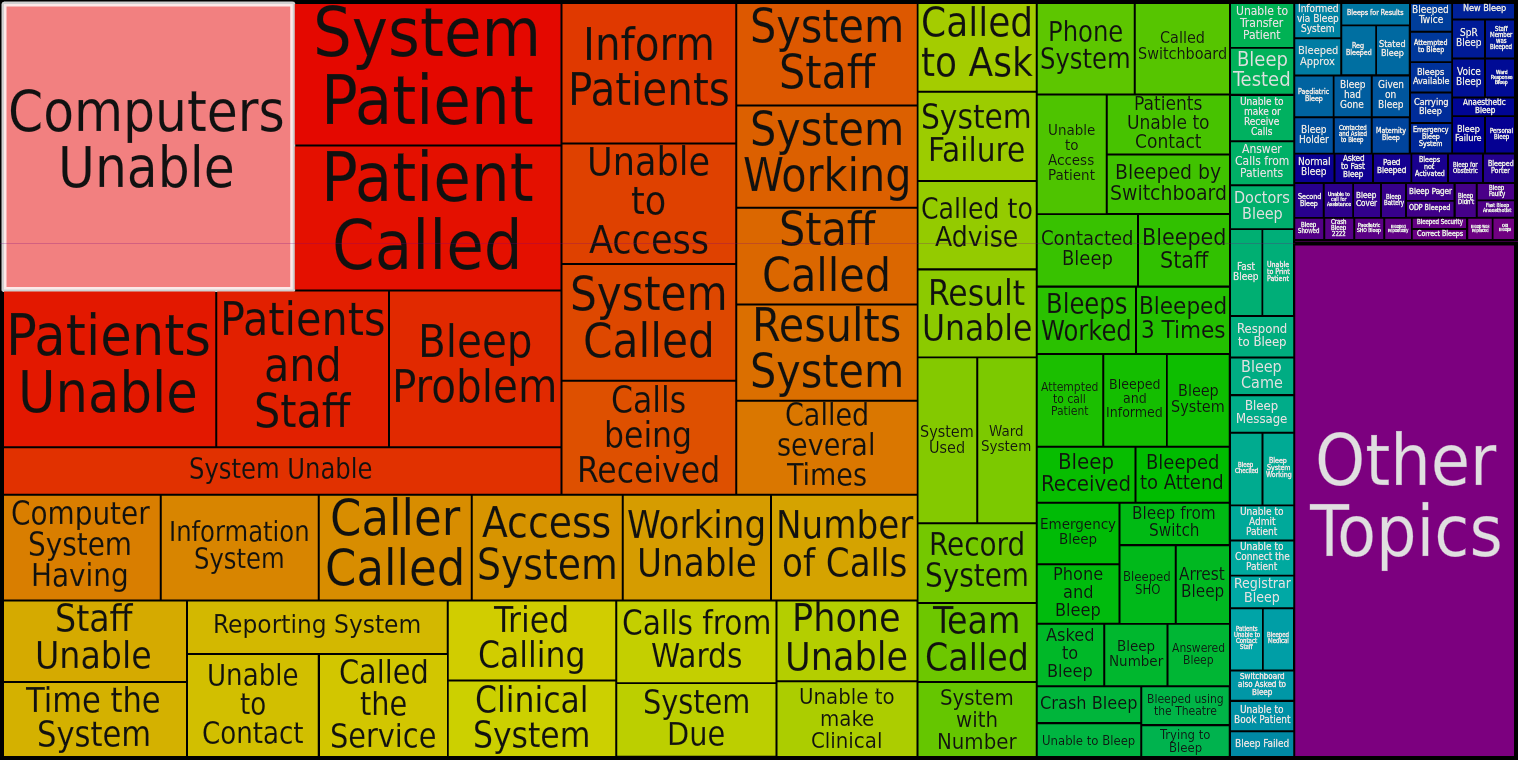
\includegraphics[width=10cm,height=7cm]{figs/lingoclustering.png}
\caption{Lingo cluster analysis of free text of 7273 patient safety incidents }\label{fig:bugsa}
\end{figure}
\end{frame}


\begin{frame}
\begin{itemize}
  \item Limitations: under-reporting and reporter ignorance
  \item `Still not fixed' and `broken again' were common strings
  \item Failing bleep systems seemed to be a major problem... (yes we're still using pagers..)
  \item Sorry substitute for having a public online issue tracker/bug reporting system
 \end{itemize}
\end{frame}	


\section{Why is it so suboptimal?}
\begin{frame}
\begin{itemize}
  \item Leadership lacks digital nous 
  \item Broken/suboptimal market (end-users lack influence, granularity problem)
  \item Structural barriers e.g archaic procurement processes, information governance, N3, IE7...
 \end{itemize}
\end{frame}	
  
\begin{frame}
  \frametitle{}   % Insert frame title between curly braces
  
\begin{figure}[htp]
\centering
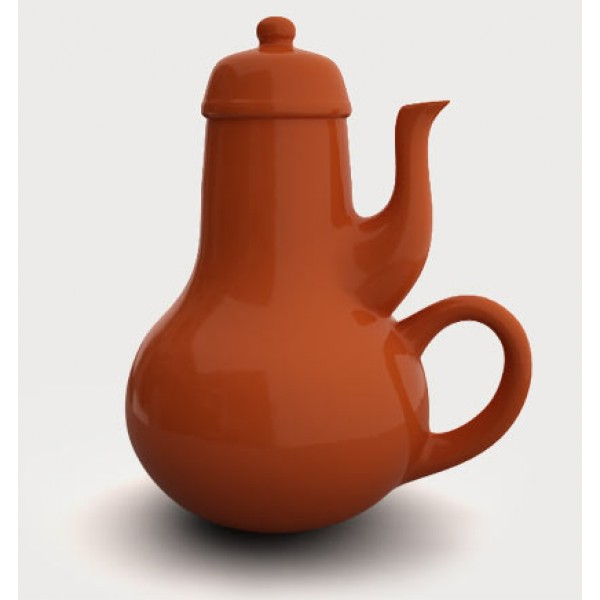
\includegraphics[width=10cm,height=7cm]{figs/badcoffeepot.jpg}
\caption{This is a user unfriendly tea pot}\label{fig:bugsa}
\end{figure}
\end{frame}
  

\section{What to do?}
\begin{frame}
\begin{itemize}
  \item Champion health promotion (citizens, patients, clinicians)
  \item Support NHS Hack Day
  \item Contribute to a real life NHS open-source, open-governance project, there exists at least one in the Real World - https://github.com/openhealthcare/opal
  (disclaimer: it's ours)
 \end{itemize}
\end{frame}	
  

\section{Thanks, questions and discussion}
\begin{frame}
  \frametitle{Questions and discussion}   % Insert frame title between curly braces

  \begin{itemize}
  \item Thoughts?
  \item Anything else I/we can/should be doing
  \item Thank-you for listening
  
  \item Contact \begin{itemize}
	 \item in-person: catch me now or later (I'm living in SeriousCamp)
         \item email: carl.reynolds@openhealthcare.org.uk
	 \item twitter: @drcjar 
	 \item web: www.carlreynolds.net / www.openhealthcare.org.uk
        \end{itemize}
 
  \end{itemize}
\end{frame}

\note{} 

%\section*{References}
%\begin{frame}
%  \frametitle{Credits and References}   % Insert frame title between curly braces

 % \begin{itemize}
 % \item I am grateful to Paul Cullinan for gifting this interesting idea to me.
 % \end{itemize}
%\end{frame}


\end{document}
